\documentclass[11pt]{bgcletter}
\usepackage{hyperref}

\name{Dr.\ Carlos A. Sierra}
\signature{ \vspace{-2cm} Carlos A. Sierra, PhD}
\email{csierra}
\telephone{6133}
\begin{document}
\begin{letter}{Dr. Takashi Asaeda\\
 Editor in Chief \\ Wetlands Ecology and Management}

\opening{Dear Dr. Aseda}
Thank you very much for your consideration of our manuscript and for the opportunity to submit a revised version. We made several changes to the manuscript based on the reviewers' comments. More prominently, we added two new sections, one describing the statistical methods used in the study, and another discussing the implications of our findings. For reproducibility and clarity in our data analysis methods, we also now provide the data and the code necessary to reproduce all results and figures. 

 In the text below, we provide answers ({\color{blue} blue font}) to all reviewers' comments ({\it italics font}). 

{\bf Reviewer 1} \\
{\it The manuscript of Volkel et al. strengthens previous findings showing that most soil carbon in mangroves is from local production. This is one of the few manuscripts I have seen for this region in Latin America, so it is regionally important. The conclusions on soil carbon origin were supported by mineralogical analyses and stable isotopes, although the stable isotope analyses was incorrectly performed. The design of the study is well conducted, although the number of samples is relatively low (n= 10 plots). The manuscript is well written. See below my detailed suggestions:}

{\color{blue} We thank the reviewer for recognizing the value of the manuscript. Although the reviewer mentions that this study has weaknesses in terms of the isotopic analysis conducted and its representativeness, we believe this is a misunderstanding and clarify these issues in the more specific comments below. }

\begin{itemize}
\item {\it L9- Is better to extrapolate to 1m, instead of 0.8m, to facility comparisons among studies (see (Kauffman and Donato, 2012)}

{\color{blue} We can easily report the values up to 1 m for basin mangroves, but for fringe mangroves soil depth does not go below 0.8 m. It would be wrong to make such an extrapolation. We therefore provide in the abstract a value up to 1 m for the basin mangroves and only up to 0.8 cm for fringe mangroves.}

\item {\it L107- Brand of EL analyser?}
{\color{blue} Elementar. Information added to the manuscript. }

\item {\it L114- Isotopes are ``values'', not signatures, they are not constant. You have to include in your end member analyses: mangrove material, riverine material, marine material (phytoplankton?). You could plot them as a triangle or analyse with mixing model. See (Fry, 2013)}

{\color{blue} We changed `signatures' to `values' as suggested by the reviewer. Please note that we used reported values for the mangrove material as end member in our analysis. We acknowledge that the isotopic analysis could be improved if more end members were available; however, we also want to point out that we not only used C isotopes to identify source contributions, but also mineralogy analyses of river and marine sediments.}

%However, at this point we cannot add a third end member to the analysis since the sampling campaign did not include mangrove material. We considered the sand samples as end members for the marine material, which help to identify inorganic contributions. We acknowledge that the isotopic analysis could be improved if more end members were available; however, we also want to point out that we not only used C isotopes to identify source contributions, but also mineralogy analyses of river and marine sediments. }

\item {\it L117- where were the samples analysed?}

{\color{blue}At the Max Planck Institute for Biogeochemistry in Jena, Germany. This information was added to the manuscript.}

\item {\it L119- What are the standards used for the isotope analyses? }

{\color{blue} The standards were Ali-j3 and Caf-j3. We added a reference were these standards are reported.}

\item {\it L134- How were the samples analysed? }

{\color{blue} We added a section on data analysis describing basic statistical analyses used in this manuscript.}

\item {\it Results \\
You need to add F, df, and p values to all your comparisons. }

{\color{blue} Done.}

\item {\it L156- Make a section on statistical analyses within the Methodology. }

{\color{blue} Done. We are also providing as supplementary material all code and data to reproduce the statistical analyses and figures reported.}

\item {\it L166- Stable isotope values are ratios compared to a standard, so it is obvious that if the value is close to zero, it means that is similar to the standard. No need to explain it. }

{\color{blue} Sentence removed as suggested.}

\item {\it L172- What about sediment deposited in the basin forest after hurricanes, storm surges? Would that contribute to higher riverine sediment in the basin forest? }

{\color{blue} This is irrelevant for our site. During the entire historical hurricane record, no hurricane have arrived to the Colombian Caribbean coast (see Figure below). This is due to the geographical location of this coast, which is protected by the northern part of the South American continent from the main tracks of Atlantic hurricanes. }

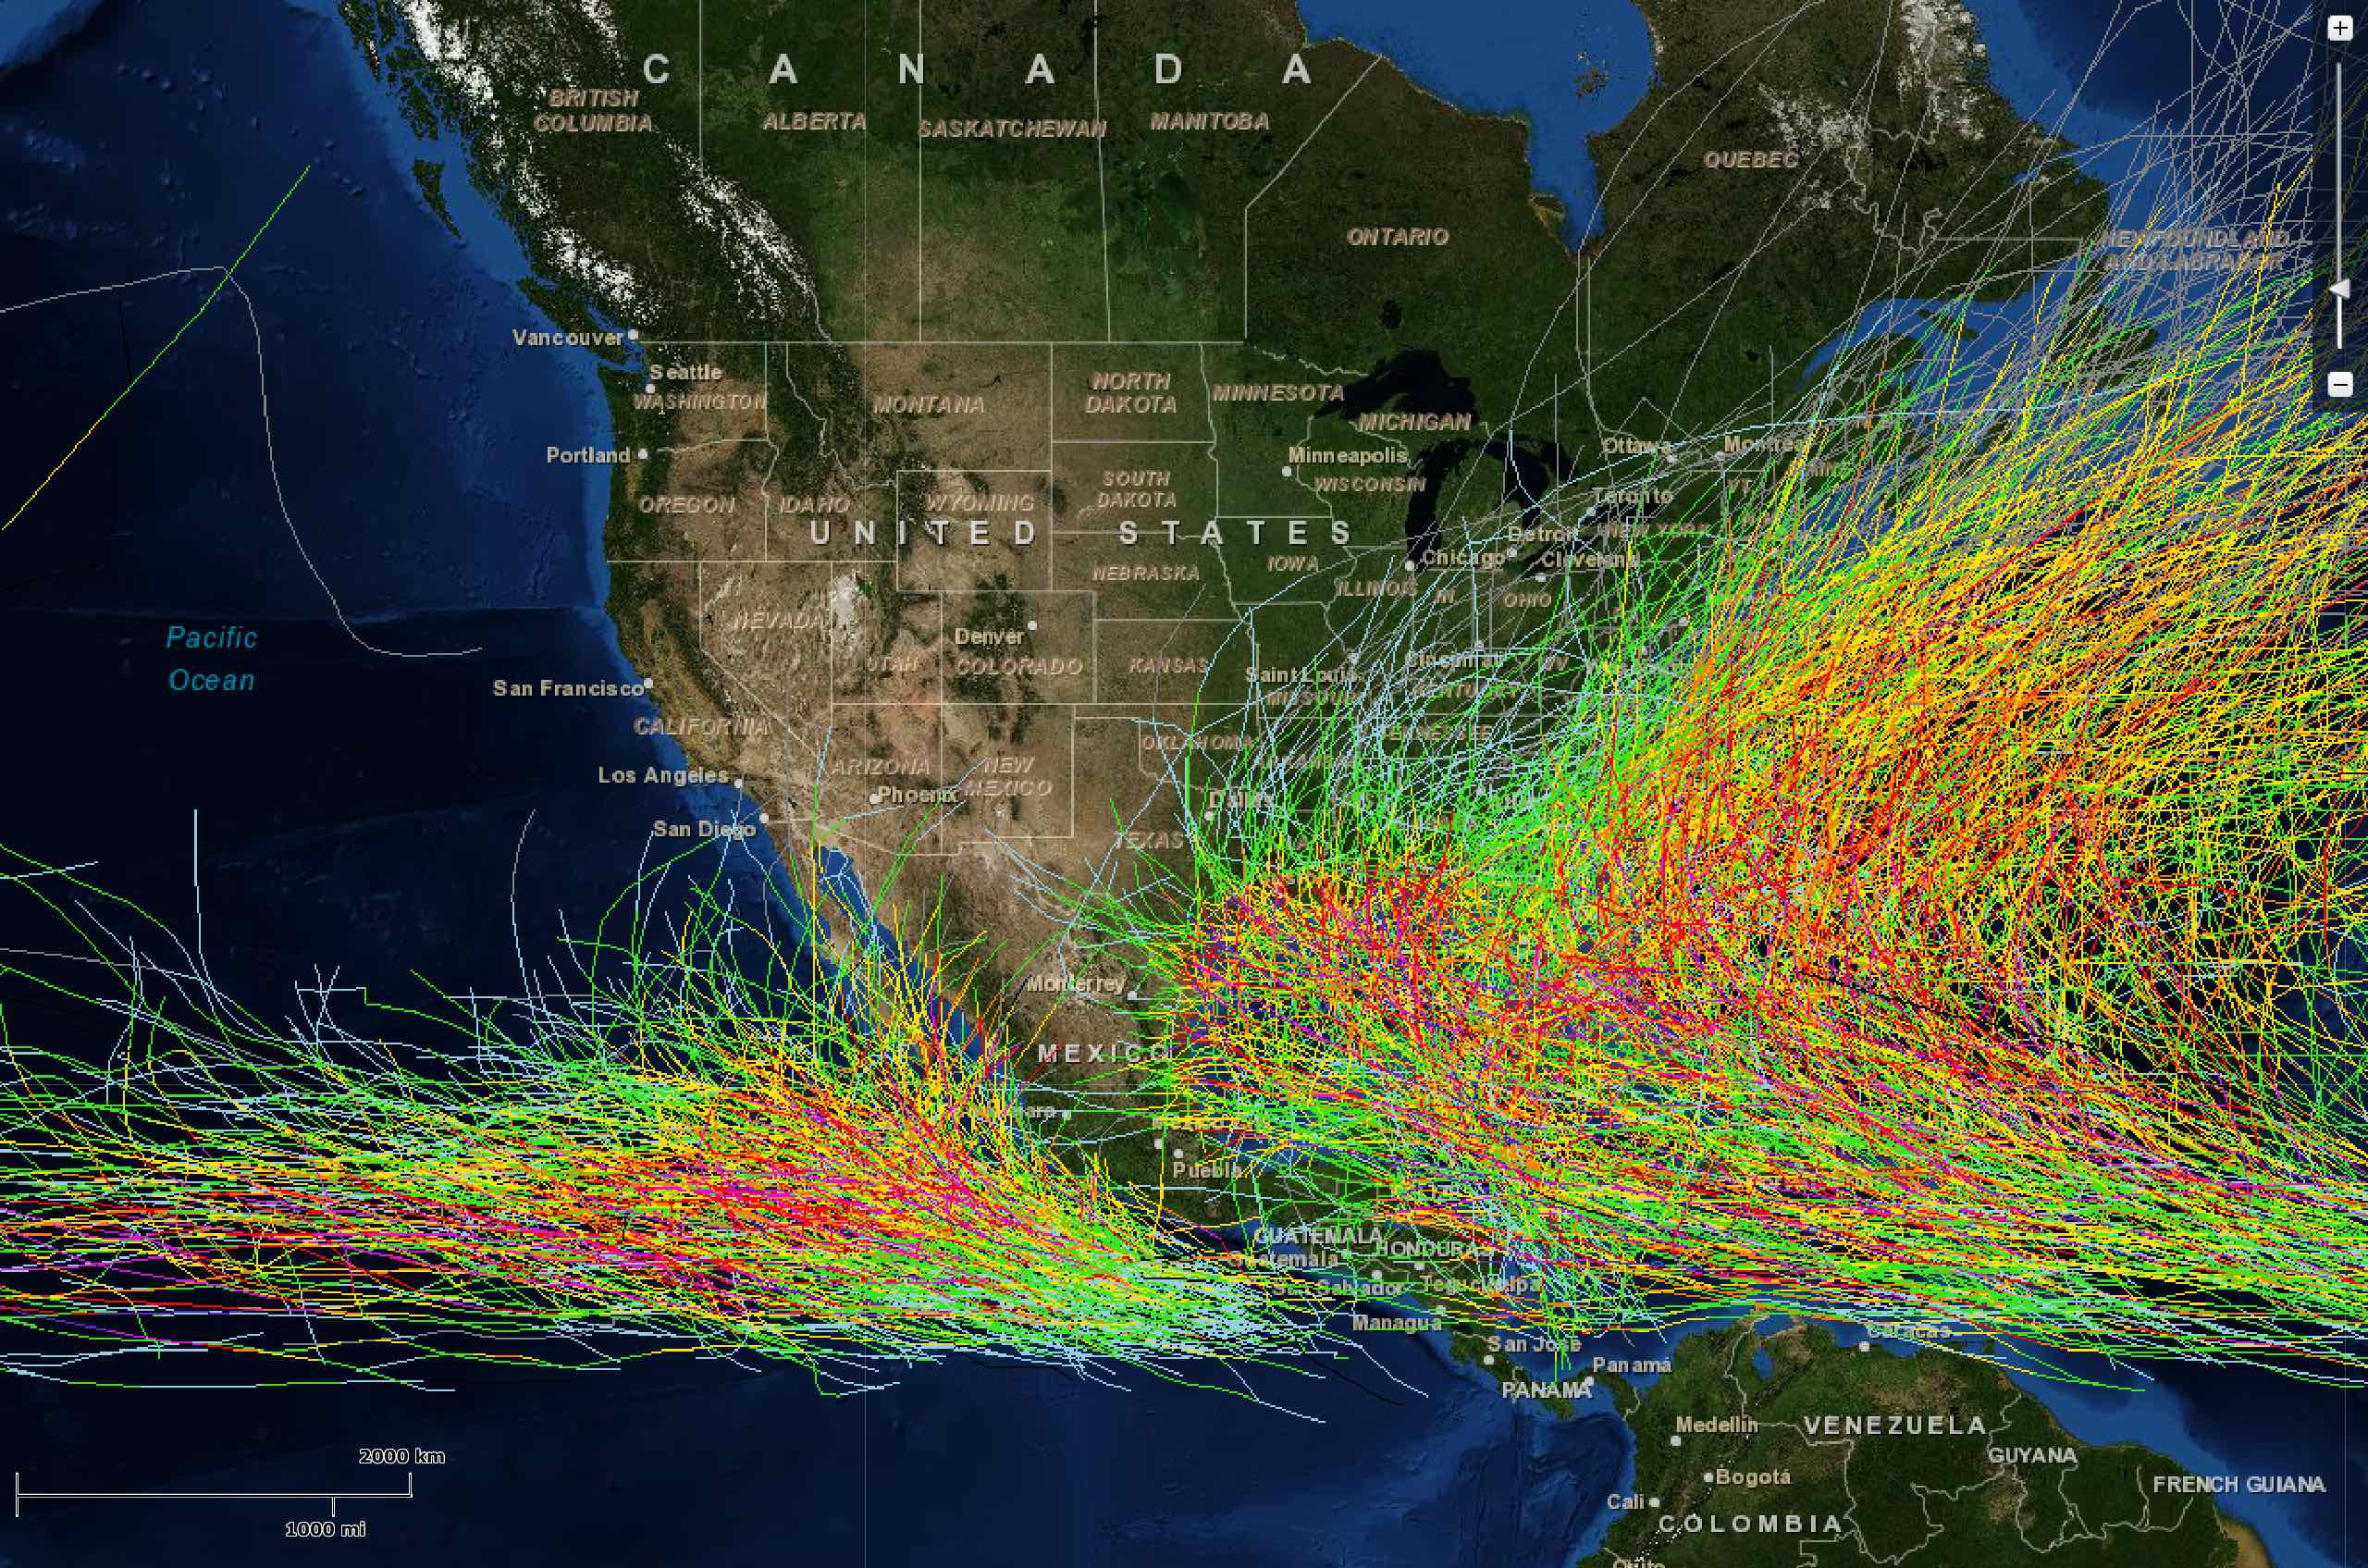
\includegraphics[scale=0.15]{noaa-hurricane-tracker.jpg}

\item {\it Fig 2- It would be more interested to have the mean values for the fringe vs basin vs sand vs river material, instead of values for each of the plots. }

{\color{blue} Figure changed as requested.}

\item {\it Fig 3- Better to call the end members `riverine' instead of `Sinu'. Need to include other end members to the analyses such as mangrove material and phytoplankton (maybe some published values ?)}

{\color{blue} We made a number of changes in this figure to improve clarity, including the issue suggested by the reviewer. Published values for other end members are provided in the text.}

\item {\it L221- This is not really interesting or relevant to this paper}

{\color{blue} Although it may not be very interesting, we consider it is relevant to report that the measured values for the sand end member are similar to those of the standard.}

\item {\it L223- And decomposition}

{\color{blue} We changed `heterotrophic consumption by microorganisms' by `decomposition' as suggested.}

\item {\it L259- $\delta$13C is not produced by anything, is just a ratio between the heavy (13C) and the light (12C) isotope. }

{\color{blue} We change `producer' by `contributor' to address this comment.}

\item {\it L266- Need to include all the relevant end members}

{\color{blue} As mentioned before, we used three end-members in our analysis. We also acknowledge that end members for phytoplankton are missing, but our analysis is complemented by the analysis of mineral composition of the sediments. }

\item {\it L357- I am not sure this is the conclusion of the manuscript. Although most of the C seems to be derived from mangroves, basin forests seem to have a higher contribution of other source, either riverine or marine? You could use the N:C values to clarify sources. }

{\color{blue} We found that soils in basin mangroves are dominated by riverine sediments; however, carbon contents in the river samples were close to zero. Instead, we found similar mineralogy among both sediments, but much larger C storage in the basin mangroves. It is well stablished that C has a large affinity to sorb in mineral surfaces of sediments, and our analysis is indicative that the in-situ derived carbon has been stabilized in this mineral surfaces. We believe this is strong evidence to reach this conclusion. }

\item {\it L367- I did not understand how the mineralogical composition facilitates dissolved carbon absorption. Regardless, it doesn't seem to matter much if most of the material is from mangrove origin as it has been shown in previous studies}

{\color{blue} The mineral composition of the sediments determines the surface area available for dissolved organic molecules to sorb. This is well known for different soils and mineral surfaces. To make this more clear, we added a number of additional references and explain this process with more detail in the text. }

\end{itemize}

{\bf Reviewer 2} \\
{\it This paper aims to study source of carbon in a mangrove-wetland complex in Colombia by exploring sediment characteristics. Although a potentially important and interesting study, it appears authors/researchers were not able to gather evidence that might be sufficient to draw the conclusions they presented. This reviewer believes that after critical revision, adding significant new information and providing additional analysis/interpretation their work could be a good addition to the literature, but in its present form, it is not fit for publication.}

{\color{blue} We thank the reviewer for recognizing the importance of this work as well as providing critical comments. We acknowledge that some information was missing in the first version of the manuscript, and we made an effort to include missing details.}

{\it This MS could benefit immensely with a clear layout of sampling plan - sampling stations/plots, mangrove types, distribution and general habitat characteristics, elaborating the logic behind the selection of sampling plots. Attributes such as water depth, tidal range, salinity, proximity to the river mouth, fresh water discharge (rainfall patterns) and tidal mixing etc should be provided. Size of estuarine complex, and annual rainfall etc can be included in study area description.}

{\color{blue} An important detail that we forgot to mention in the submitted version is that this study was part of a much larger project in which a number of plots were stablished previously to estimate carbon stocks in the area. We did not selected the plots ourselves, but rather sampled the set of existing plots. Criteria for plot selection are described in other publications and we refer to them in the new version of the manuscript. }

{\it Also, Figure 1 (map of study location) indicates that river Sinu flows almost 10-12 km west of the sampling region. There is not clear suggestion in the figure or text that samples sites receive waters from River Sinu. This reviewer is somewhat perplexed and unable to understand the hypothesis and choice of the study design. Perhaps some clarification and effort in explaining this via text and figures would be beneficial for the readers.}

{\color{blue} We acknowledge that this point may not have been well explained in the area description section of the previous version of the manuscript. The Sin\'u River changed its course in 1938, and before this year it discharged in the study area. This is well documented in Serrano (2004), and we provide now a better explanation in the description of the study site.}

{\it Some important information is missing in the laboratory analysis section. For this entire section there is no reference/no citation. This reviewer encourages authors to cite appropriate methods that were followed for analysis, and include all necessary and important details.}

{\color{blue} We added necessary citations regarding the different methods used.}

{\it For calculating carbon storages in the sampled sites, bulk density of only one fringe site (P21) and one basin site (C4) was used for all plots. There is a large amount of spatial variability in soils even at small resolution and it is important to use site specific bulk density to calculate site specific storages. This reviewer has a serious reservation against this methodology.}

{\color{blue} Please note the extreme differences in bulk density between the two mangrove types reported in Table 1. While basin mangroves have a bulk density of around 1.1, fringe mangroves are around 0.1 g cm$^{-3}$. We obtained similar results in a previous study that included more replicates (Bolivar 2015), and the numbers reported here simply confirm previous measurements. It is unlikely that these differences are due to spatial variability within mangrove types. In fact, these differences in bulk density are an inherent characteristic of the different mangrove types. The fringe mangroves are stablished in the old Sin\'u river delta sediments, while the fringe mangroves advance the cost line and establish over coastal sands. }

{\it This methods section does not include any description how data was analyzed. No statistical information is provided. What programs were used. Whether any tests for normalcy were performed? It is a standard practice to include such information in the MS. }

{\color{blue} We added a new section describing the statistical procedures and the software used. In addition, we provide the code and data to reproduce all results.}

{\it This reviewer believes that the discussion section of this MS should be revised with more critical inputs, highlighting the new addition to this field. This reviewer commends authors for tedious field work and many hours of data entry and subsequent analysis, but it becomes difficult to see value of this research unless a more rigorous and through discussion is presented. The researchers could also report the broader implications of their research… i.e. How this understanding would be beneficial and for whom.}

{\color{blue} Thanks for the recommendation. We added a paragraph to the discussion about the broader implications of this study.}

{\it There are multiple incidences of discrepancies in sentence syntax and complex sentence formulation that diminishes readability and clarity of the text. This reviewer has suggested moving around text, and rewriting sentences to impart clarity. Such corrections will improve paper's readability and should be relatively straight-forward to fix. }

{\color{blue} Thanks for pointing this out. We edited the text in several parts to reduce sentence complexity and improve clarity.}

\vspace{2em}
{\bf Comments by reviewer 2 on pdf version of the article} \\
The pdf version of the article provided by the reviewer contained a large number of highlighted text, comments, and strikethrough text. We provided below answers to the comments, and the strikethrough text was removed from the manuscript. However we did not performed any action on the highlighted text since there was no indication by the reviewer on the reason the text was highlighted. 

{\color{blue} Can you provide an approximate size of this estuarine lagoon complex?} \\
{\it The total area is 5,098 ha. We added this value to the site description section. }

{\color{blue} how about Crystalline iron oxides? } \\
{\it The oxalate extraction dissolves mostly poorly crystalline iron oxides, while the dithionite extraction removes the crystalline Fe oxides. We added this to the text. }

{\color{blue} Figure 4, About 85\% is Aragonite. That also clearly suggests CaCO3 presence. }
{\it Yes, this is correct and we point it out in the main text as well. }

{\color{blue} Ln. 240. Consider rewriting. Doesn't convey meaning clearly} \\
{\it Sentence rewritten as suggested.}

{\color{blue} Ln 303. Looks like there is something missing here. You can provide more information here to build up an explanation for your observation. } \\
{\it This sentence was removed from the latest version of the manuscript because it does not add useful information for the message we want to convey. }

\vspace{2em}
We hope this new version adequately addresses reviewer's comments and it is now suitable for publication.

\closing{Sincerely, \\
 \includegraphics[scale=0.7]{../../../../Documents/Personal/firma.jpg}
 }
 \end{letter}

 \end{document}
